\section{图片}


论文中不可避免要插入图片。图片可以分为矢量图与位图。位图推荐使用 \verb|jpg,png| 这两种格式,避免使用 \verb|bmp| 这类图片,容易出现图片插入失败这样情况的发生。矢量图一般有 \verb|pdf,eps| ,推荐使用 \verb|pdf|  格式的图片,尽量不要使用 \verb|eps| 图片,理由相同。

注意图片的命名,避免使用中文来命名图片,可以用英文与数字的组合来命名图片。避免使用\verb|1,2,3| 这样顺序的图片命名方式。图片多了,自己都不清楚那张图是什么了,命名尽量让它有意义。下面是一个插图的示例代码。
\begin{figure}[!h]
    \centering
    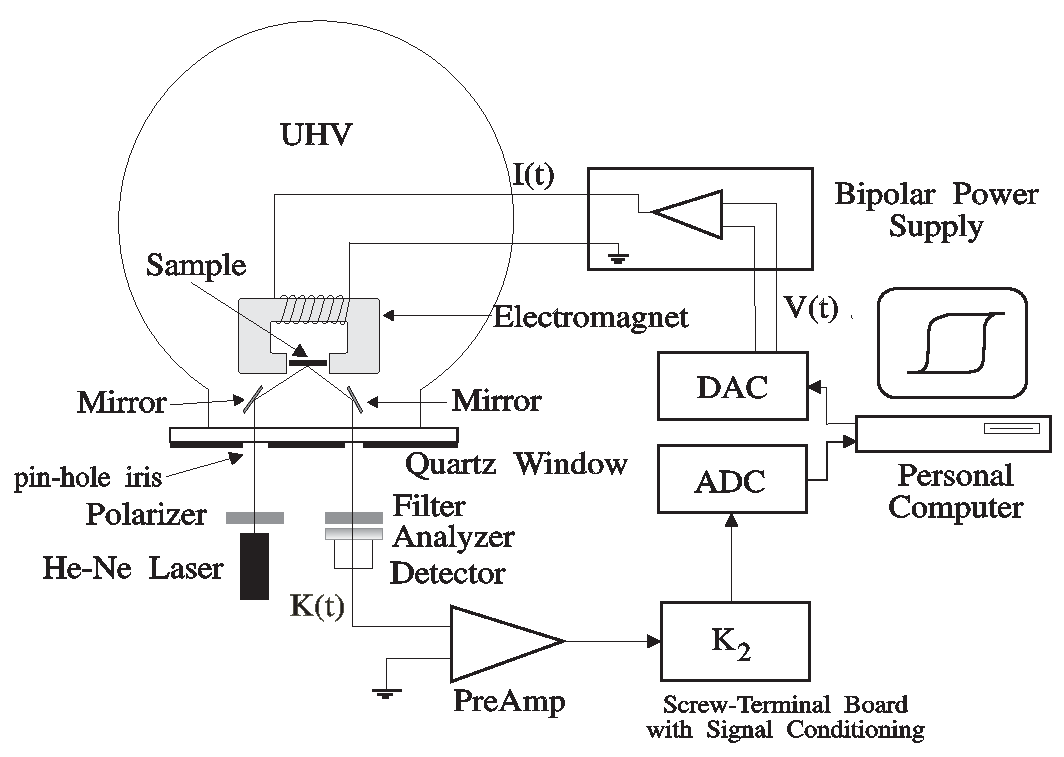
\includegraphics[width=.6\textwidth]{figures/smokeblk.pdf}
    \caption{电路图}
    \label{figures:smokeblk.pdf}
\end{figure}

注意 \verb|figure| 环境是一个浮动体环境,图片的最终位置可能会跑动。\verb|[!h]| 中的 \verb|h| 是 here 的意思, \verb|!| 表示忽略一些浮动体的严格规则。另外里面还可以加上 \verb|btp| 选项,它们分别是 bottom, top, page 的意思。只要这几个参数在花括号里面,作用是不分先后顺序的。page 在这里表示浮动页。

\verb|\label{fig:circuit-diagram}| 是一个标签,供交叉引用使用的。图片是自动编号的,比起手动编号,它更加高效。\verb|\cref{label}| 由 \verb|cleveref| 宏包提供,比普通的 \verb|\ref{label}| 更加自动化。 \verb|label| 要确保唯一,命名方式推荐用图片的命名方式。

图片并排的需求解决方式多种多样,下面用 \verb|minipage| 环境来展示一个简单的例子。注意,以下例子用到了 \verb|subcaption| 命令,需要加载 subcaption 宏包。

\begin{figure}
    \centering
    \begin{minipage}[c]{0.3\textwidth}
        \centering
        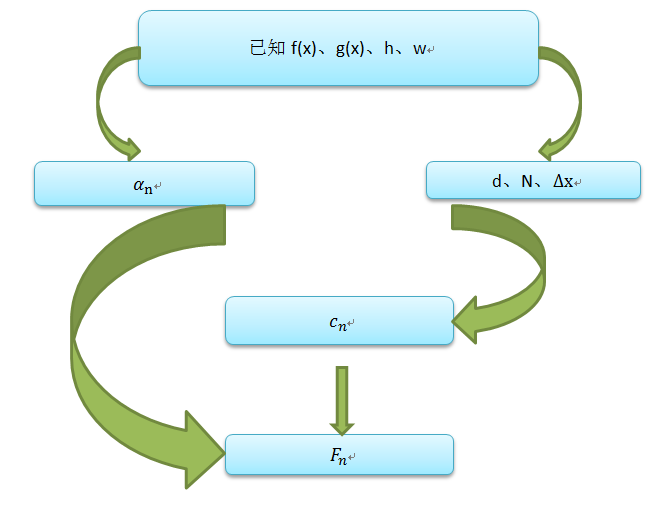
\includegraphics[width=0.95\textwidth]{figures/f1.png}
        \subcaption{流程图}
        \label{fig:sample-figure-a}
    \end{minipage}
    \begin{minipage}[c]{0.3\textwidth}
        \centering
        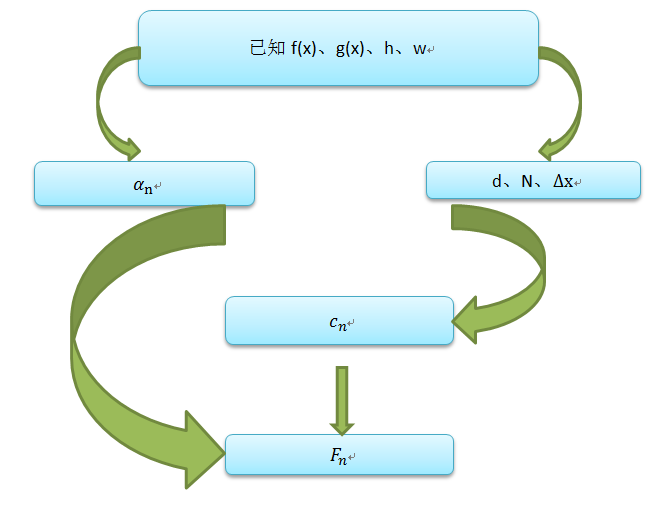
\includegraphics[width=0.95\textwidth]{figures/f1.png}
        \subcaption{流程图}
        \label{fig:sample-figure-b}
    \end{minipage}
    \begin{minipage}[c]{0.3\textwidth}
        \centering
        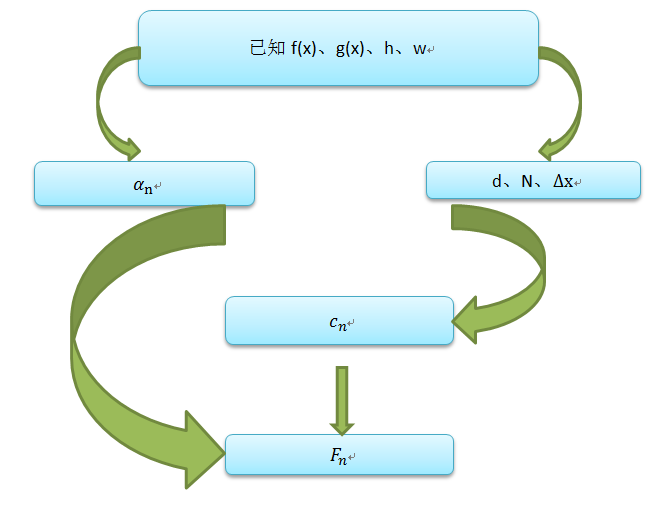
\includegraphics[width=0.95\textwidth]{figures/f1.png}
        \subcaption{流程图}
        \label{fig:sample-figure-c}
    \end{minipage}
    \caption{多图并排示例}
    \label{fig:sample-figure}
\end{figure}

这相当于整体是一张大图片,大图片引用是\cref{fig:sample-figure},子图引用别分是\cref{fig:sample-figure-a}、\cref{fig:sample-figure-b}、\cref{fig:sample-figure-c}。

如果原本两张图片的高度不同,但是希望它们缩放后等高的排在同一行,参考这个例子:
\begin{figure}[H]
    \centering
    \begin{minipage}[c]{0.4\textwidth}
        \centering
        
\includegraphics[height=0.2\textheight]{figures/cat.pdf}
        \subcaption{一只猫}
    \end{minipage}
    \begin{minipage}[c]{0.4\textwidth}
        \centering
        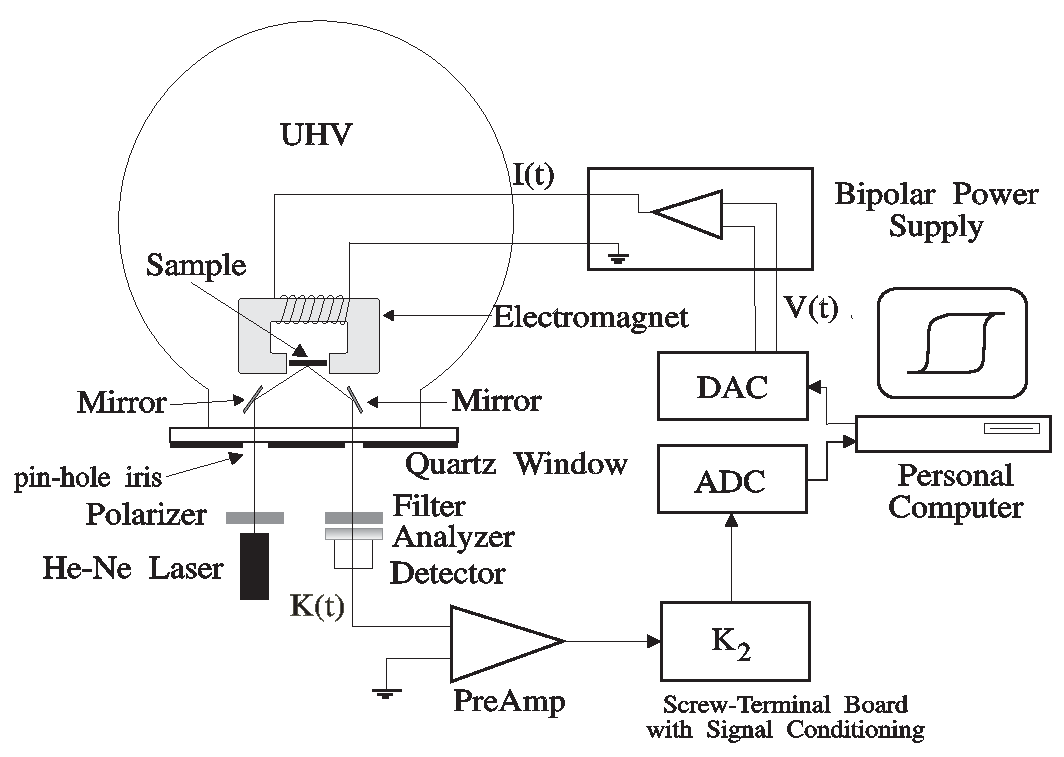
\includegraphics[height=0.2\textheight]{figures/smokeblk.pdf}
        \subcaption{电路图}
    \end{minipage}
    \caption{多图并排示例}
\end{figure}
